\section{Energiespeicher}

Die gesamte Energiespeicherung wird in einzelne Komponenten aufgeteilt, wobei Abbildung \ref{fig:blockschaltbild} einen groben Überblick zum Aufbau gibt.

\begin{figure}[H]
	\begin{center}
		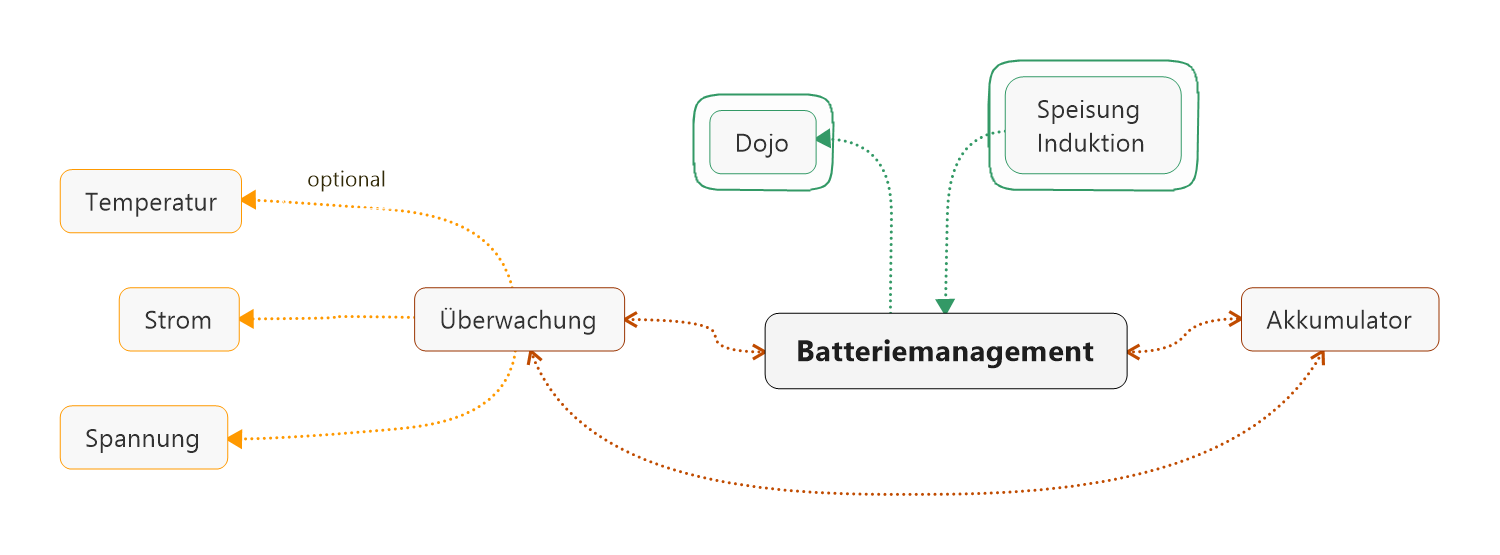
\includegraphics[width=160mm]{data/Batteriemanagement.png}
		\caption{Blockschaltbild Energiespeicherung} %picture caption
		\label{fig:blockschaltbild}
	\end{center}
\end{figure}

Das Batteriemanagement bildet den Kern der gesamten Einheit und übernimmt, wie der Name schon sagt, das gesamte Management zwischen Batterie und Speisung. Der Akkumulator wird durch Überwachungsparameter wie Strom und Spannung kontrolliert und übernimmt die gesamte Energieversorgung des Dojos. Die Überwachung der Temperatur ist lediglich notwendig falls eine Schnellladefunktion implementiert wird. Dieses Zusatzfeature bleibt aber ein Wunschziel und wird in erster Linie nicht weiterverfolgt.

\subsection{Speicher}
Der Akkumulator besteht aus Lithium-Ionen Zellen, welche zusammen eine Spannung von 3.6V aufweisen. Aufgrund der 17mm Innendurchmesser des Dojos, sind die Abmessungen und somit auch die Auswahl an möglichen Energiespeichern relativ fix gegeben. Die notwendige Kapazität kann durch die zwei Faktoren Zeit und Energieverbrauch berechnet werden. Die Betriebszeit sollte hierbei einen Aufenthalten ohne Ladezyklus ermöglichen. Durchschnittlich haben Museen an einem Tag rund 7h geöffnet, wobei mit einem durchschnittlichen Aufenthalt von drei bis vier Stunden pro Person gerechnet wird. Die Betriebszeit des Dojos ermöglicht eine Betriebszeit von fünf Stunden, wobei durch Ladezyklen zwischen den Besuchen eine ganztägiger Betrieb ermöglicht wird. Um dies zu veranschaulichen, gibt nachfolgende Abbildung \ref{fig:Ladezyklus Dojo} einen Einblick ins Konzept.

\begin{figure}[H]
	\begin{center}
		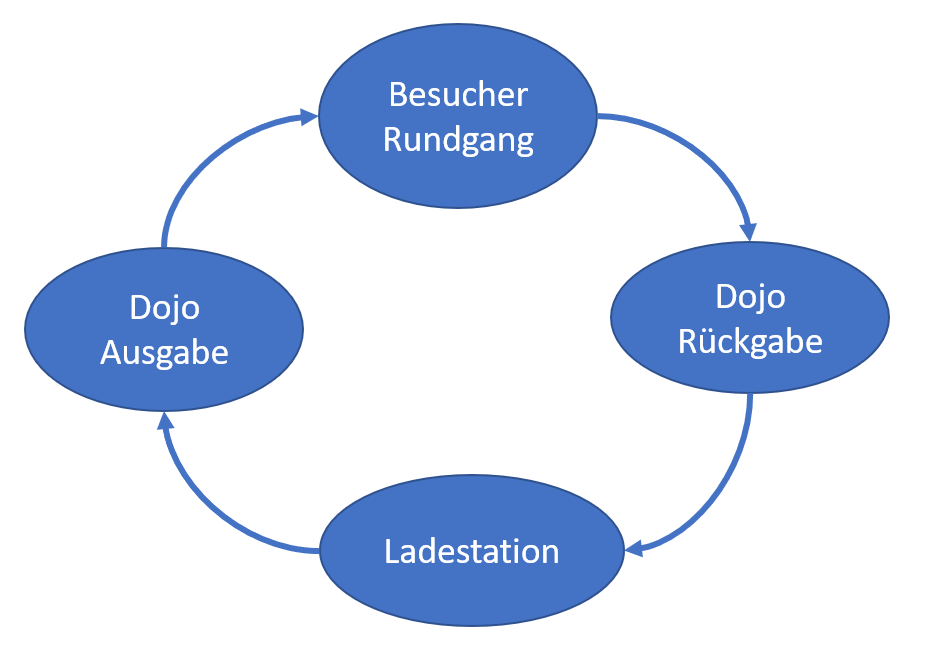
\includegraphics[width=120mm]{data/LadezyklusDojo.png}
		\caption{Ladezyklus Dojo} %picture caption
		\label{fig:Ladezyklus Dojo}
	\end{center}
\end{figure}

Wie bereits oben beschrieben, beträgt die Betriebszeit eines durchschnittlichen Rundganges rund drei bis vier Stunden. Sobald die Rückgabe erfolgt ist, wird das Dojo in die Ladebuchse gesteckt wobei immer diese Dojos rausgegeben werden, welche sich am längsten in der Ladestation befinden. Bei einer Stückzahl welche grösser ist als die Besucherzahl, erlaubt dies einen lückenlosen Betrieb.
Die notwendige Kapazitätsberechnung wird durch Formel \ref{fig:kapazitaet} beschrieben. Die maximale Leistung des Dojos lässt sich durch Leistung des Knochenschallgebers und des Microcontrollers beschreiben. Alle anderen Komponenten können durch ihren geringen Betriebsstrom vernachlässigt werden. Der Knochenschallgeber weist eine durchschnittliche Leistung von 0.35 Watt auf. Die Rechnung erfolgt mit einem Wert von rund 0.5W und einer Betriebszeit von rund 80$\%$. Die Microcontrollerleistung lässt sich durch den Radio Strom (7.5mA) und einigen Mikroampere Systemstrom (gesamthaft ca. 100 $\mu$ A) multipliziert mit der Systemspannung von 3.6V bestimmen. Nachfolgende Formel \ref{fig:LeistungMC} zeigt die Berechnung der Microcontrollerleistung und Formel \ref{fig:kapazitaet} zeigt die Kapazitätsabschätzung.

\begin{equation}
P_{MC}=U\cdot I_{MC}
\label{fig:LeistungMC}
\end{equation}
\begin{equation}
Q=\frac{\left(t\cdot 0.8\cdot P_{Kn}\right)+\left(t\cdot P_{MC}\right)}{U}=\frac{\left(5h\cdot 0.8\cdot 0.5W\right)+\left(5h\cdot 3.6V\cdot 7.6mA\right)}{3.6V}=0.594Ah
\label{fig:kapazitaet}
\end{equation}

Die geforderte Kapazität liegt gemäss Formel \ref{fig:kapazitaet} bei 0.594Ah. Unabhängig von der Grösse der Batterie ist der Schutz vor äusseren Einflüssen. Hierbei kann mittels einer gezielten Überwachung die Lebensdauer der Batterie wesentlich verlängert und die anfallenden Nebenkosten vermindert werden. Diese Thematik wird im nachfolgenden Unterkapitel \ref{Überlade und Entladeschutz} genauer erläutert.
                                         
\subsection{Überlade und Entladeschutz}  \label{Überlade und Entladeschutz}

Der Überlade- und Entladeschutz, besteht aus der Überwachung des Ladeprozesses wie auch der Signalisation bei Unterschreitung einer definierten Spannungsschwelle. Die Überwachung beim Ladezyklus erfolgt durch eine Spannungsüberwachung welche wie in Abbildung \ref{fig:Ladekurve Li-Ion Akku} ersichtlich erfolgt. Hierbei ist gut ersichtlich, dass die letzten ca. 20\% der Aufladung auf einem Spannungslevel von 4.2V erfolgen. Für die Regelung wird ein Batterielade-IC vom Typ MCP73831T verwendet.
Während dem Ladevorgang kann hierbei zusätzlich 1 LED für die Signalisation des Ladevorgangs angesteuert werden. Für die Entladeüberwachung kann die Spannung der Batterie auf zwei Pins am Microcontroller angeschlossen und auf dem Microcontroller selber überwacht werden. Dies gewährleistet dass bei niedriger Spannung das gesamt System heruntergefahren und so der Akku vor Tiefentladung geschützt werden kann.

\begin{figure}[H]
	\begin{center}
		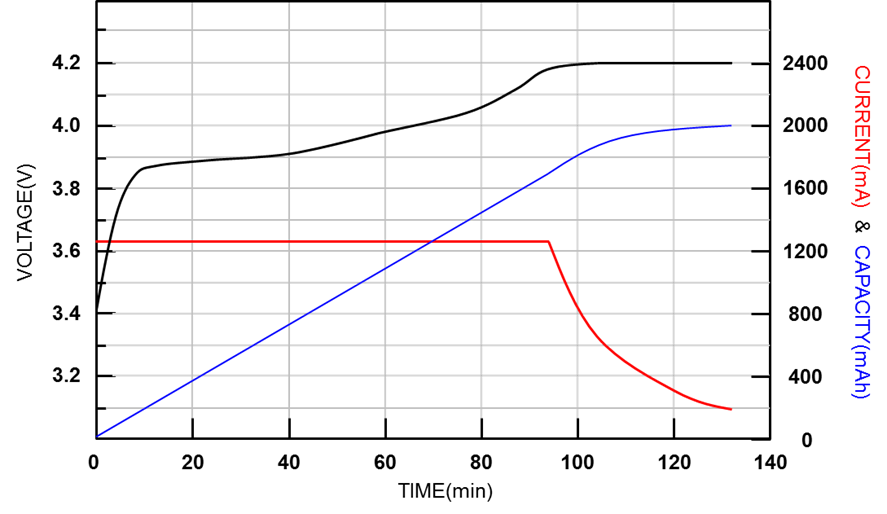
\includegraphics[width=120mm]{data/LadekurveLiIon.png}
		\caption{Blockschaltbild Energiespeicherung} %picture caption
		\label{fig:Ladekurve Li-Ion Akku}
	\end{center}
\end{figure}
